\documentclass{article}

% if you need to pass options to natbib, use, e.g.:
%     \PassOptionsToPackage{numbers, compress}{natbib}
% before loading neurips_2026

% The authors should use one of these tracks.
% Before accepting by the NeurIPS conference, select one of the options below.
% 0. "default" for submission
\usepackage{neurips_2026}
% the "default" option is equal to the "main" option, which is used for the Main Track with double-blind reviewing.
% 1. "main" option is used for the Main Track
 % \usepackage[main]{neurips_2026}
% 2. "position" option is used for the Position Paper Track
%  \usepackage[position]{neurips_2026}
% 3. "eandd" option is used for the Evaluations & Datasets Track
 % \usepackage[eandd]{neurips_2026}
 % if you want to opt-in for a de-anomymized submission (not recommended, but OK):
 %\usepackage[eandd, nonanonymous]{neurips_2026}
% 4. "creativeai" option is used for the Creative AI Track
%  \usepackage[creativeai]{neurips_2026}
% 5. "sglblindworkshop" option is used for the Workshop with single-blind reviewing
 % \usepackage[sglblindworkshop]{neurips_2026}
% 6. "dblblindworkshop" option is used for the Workshop with double-blind reviewing
%  \usepackage[dblblindworkshop]{neurips_2026}

% After being accepted, the authors should add "final" behind the track to compile a camera-ready version.
% 1. Main Track
 % \usepackage[main, final]{neurips_2026}
% 2. Position Paper Track
%  \usepackage[position, final]{neurips_2026}
% 3. Evaluations & Datasets Track
 % \usepackage[eandd, final]{neurips_2026}
% 4. Creative AI Track
%  \usepackage[creativeai, final]{neurips_2026}
% 5. Workshop with single-blind reviewing
%  \usepackage[sglblindworkshop, final]{neurips_2026}
% 6. Workshop with double-blind reviewing
%  \usepackage[dblblindworkshop, final]{neurips_2026}
% Note. For the workshop paper template, both \title{} and \workshoptitle{} are required, with the former indicating the paper title shown in the title and the latter indicating the workshop title displayed in the footnote.
% For workshops (5., 6.), the authors should add the name of the workshop, "\workshoptitle" command is used to set the workshop title.
% \workshoptitle{WORKSHOP TITLE}

% "preprint" option is used for arXiv or other preprint submissions
% \usepackage[preprint]{neurips_2026}

% to avoid loading the natbib package, add option nonatbib:
%    \usepackage[nonatbib]{neurips_2026}

\usepackage[utf8]{inputenc} % allow utf-8 input
\usepackage[T1]{fontenc}    % use 8-bit T1 fonts
\usepackage{hyperref}       % hyperlinks
\usepackage{url}            % simple URL typesetting
\usepackage{booktabs}       % professional-quality tables
\usepackage{amsfonts}       % blackboard math symbols
\usepackage{nicefrac}       % compact symbols for 1/2, etc.
\usepackage{microtype}      % microtypography
\usepackage{xcolor}         % colors
\usepackage{graphicx}
\usepackage{amsmath}

\graphicspath{{figures}}

\newtheorem{assumption}{Assumption}
\newtheorem{theorem}{Theorem}
\newtheorem{lemma}[theorem]{Lemma}
\newtheorem{corollary}[theorem]{Corollary}
\newtheorem{definition}[theorem]{Definition}
\newtheorem{remark}{Remark}

% Note. For the workshop paper template, both \title{} and \workshoptitle{} are required, with the former indicating the paper title shown in the title and the latter indicating the workshop title displayed in the footnote. 
\title{Curvature-Subspace Criteria for Local Loss-Landscape Stabilization}


% The \author macro works with any number of authors. There are two commands
% used to separate the names and addresses of multiple authors: \And and \AND.
%
% Using \And between authors leaves it to LaTeX to determine where to break the
% lines. Using \AND forces a line break at that point. So, if LaTeX puts 3 of 4
% authors names on the first line, and the last on the second line, try using
% \AND instead of \And before the third author name.


\author{%
  Nikita Kiselev \\
  Moscow Institute of Physics and Technology, Russia \\
  \texttt{kiselev.ns@phystech.edu} \\
  \And
  Andrey Grabovoy \\
  Moscow Institute of Physics and Technology, Russia \\
  \texttt{grabovoy.av@phystech.edu}
}


\begin{document}


\maketitle


\begin{abstract}
    % Scaling laws of modern deep neural networks are used for compute-optimal model and data size increasing. They tend to be highly valitated in practice, however theoretical foundations of them is poorly explored. In this paper, we propose a new foundational framework of loss landscape stabilization, in which adding new training samples is observed to merely change the loss surface in local minima neighborhoods. We show that previously explored one-point and squared criteria cannot fully describe the local behaviuor of the loss function, and thus propose new subspace-squared criterion, which is calculated in principal Hessian subspace. Empirial results show that subspace criteria depends on the choice of their basis, and that proposed one has the most information about the loss curvature. We explore three different algorithms for this criterion estimation in practice, and show effectiveness and robustntess of them in the neighbourhood, where quadratic approximation is valid. We also check application of proposed framework for sample size estimation problem.
    Deep neural loss landscapes are highly anisotropic: much of their meaningful local curvature is concentrated in a small number of directions. We study how such landscapes stabilize as the training set grows one sample at a time. Previous work introduced pointwise and full-space mean-squared criteria for local landscape increments, but did not place them in a unified framework and did not exploit local curvature structure, potentially averaging the signal over many weakly informative directions. We introduce a curvature-aware subspace criterion that probes local landscape change in the leading eigenspace of the empirical Hessian near a trained solution. Under a local quadratic model, we show that this criterion preserves the same mean-squared convergence order as the full-space criterion, with curvature dependence governed by the subspace dimension rather than the ambient parameter dimension. We also derive a spectral interpretation under an additional stable-eigenspace assumption and describe scalable estimators based on Hessian--vector products, subspace Monte Carlo, and quadratic proxy evaluation. Experiments on a nanochat decoder-only transformer show that the Gaussian-moment proxy estimator faithfully tracks the direct criterion across subspace dimensions $D\in[1,100]$ and perturbation scales within the valid quadratic regime ($\sigma\lesssim10^{-3}$), while diverging outside it. The proxy is approximately $18{,}000\times$ faster than direct Monte Carlo in the evaluation stage after subspace construction. These results position the proposed criterion as a well-defined curvature-aware observable within a unified framework for local landscape stabilization and clarify the current limitations of this observational design.
\end{abstract}

\section{Introduction}\label{sec:intro}

\begin{figure}[t]
  \centering
  \begin{minipage}[t]{0.48\linewidth}
    \centering
    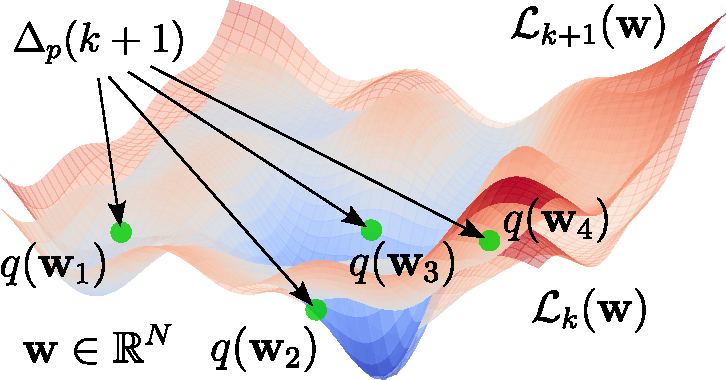
\includegraphics[width=\linewidth]{criterion_general.pdf}\\[0.3em]
    \small (a) Unified loss landscape stabilization criterion $\Delta_p$ with probing distribution $q(\mathbf{w})$
  \end{minipage}\hfill
  \begin{minipage}[t]{0.48\linewidth}
    \centering
    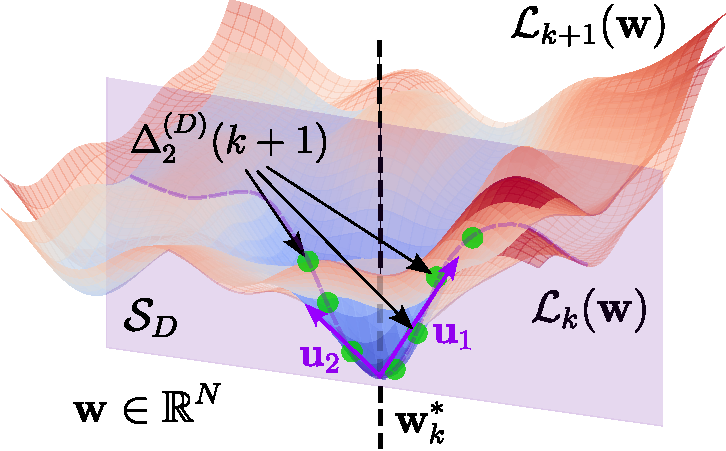
\includegraphics[width=\linewidth]{criterion_squared_subspace.pdf}\\[0.3em]
    \small (b) Principal Hessian subspace $\mathcal{S}_D$ squared criterion $\Delta_2^{(D)}$
  \end{minipage}
  \caption{\textbf{Loss landscape stabilization criteria.} (a) General framework for convergence observation with arbitrary probing distribution $q(\mathbf{w})$, and (b) Curvature-aware criterion, which capture loss increment field on a principal Hessian subspace along top-curvature directions.}
  \label{fig:overview}
\end{figure}

Training in deep learning depends not only on the value of the empirical risk at a solution, but also on the local geometry of the loss surface around that solution.
A large empirical literature studies this geometry through loss-landscape visualizations, Hessian spectra, and local sharpness, showing that curvature in modern neural networks is highly anisotropic: a relatively small number of directions often carry most of the meaningful second-order structure, while much of parameter space is weakly curved or nearly flat~\citep{li2018visualizing,sagun2017hessian,ghorbani2019investigation,papyan2019fullspectrum,xu2024mining}.
This raises a natural question under sample growth: as training examples are added one by one, how does the local empirical landscape change near a trained solution, and how should that change be observed?

Classical statistical learning theory studies convergence of empirical risk to population risk~\citep{vapnik1998statistical,shalev2014understanding}, and algorithmic stability bounds the sensitivity of learned predictors to perturbations of the training set~\citep{bousquet2002stability,feldman2019high,bousquet2020sharper}.
These frameworks are foundational, but they do not directly describe how local geometric quantities---such as gradients, Hessians, and their leading eigenspaces---change when one additional sample is incorporated.
More recently,~\citet{author:delta1,author:delta2} introduced local criteria for the increment $\mathcal L_{k+1}(\mathbf w)-\mathcal L_k(\mathbf w)$ near a minimizer $\mathbf w_k^*$ of the $k$-sample empirical risk.
In particular, the one-point criterion $\Delta_1$ yields $\mathcal O(k^{-1})$ decay, while the full-space mean-squared criterion $\Delta_2$ yields $\mathcal O(k^{-2})$ decay.

In this paper, we place such criteria in a unified framework.
The increment $\mathcal L_{k+1}(\mathbf w)-\mathcal L_k(\mathbf w)$ is a scalar field over parameter space, and any aggregated criterion for it depends not only on the aggregation order, but also on the perturbations used to probe local change.
This makes local landscape stabilization an \emph{observational} problem as well as a convergence problem.
Within this framework, previously studied pointwise and isotropic criteria appear as special cases corresponding to different probing laws, and the choice of probing distribution becomes part of the scientific question rather than merely part of the estimator.

We study a curvature-aware specialization of this framework: the \emph{subspace mean-squared criterion} $\Delta_2^{(D)}$, illustrated in Fig.~\ref{fig:overview}, which restricts Gaussian perturbations to the top-$D$ eigenspace of the empirical Hessian $\mathbf H^{(k)}(\mathbf w_k^*)$.
The purpose of this restriction is not merely dimensionality reduction, but geometry-aligned probing of the increment field near a trained solution.
Thus, $\Delta_2^{(D)}$ should be read as a curvature-aware observable of local landscape stabilization.

Our theoretical analysis studies the increment field near $\mathbf w_k^*$ under a local quadratic model.
We derive a low-dimensional representation of the subspace criterion and show that $\Delta_2^{(D)}$ preserves the same mean-squared $\mathcal O(k^{-2})$ decay as the full-space criterion, with a curvature-dependent term governed by the subspace dimension $D$ rather than the ambient dimension $N$.
Under an additional stable-eigenspace assumption, the compressed Hessian difference admits a spectral closed form in terms of leading eigenvalue increments.
The theory is therefore not a justification for using a subspace in general, but a local guarantee for this particular curvature-aware design.

We also develop scalable estimators for $\Delta_2^{(D)}$ based on Hessian--vector products, top-$D$ eigenspace extraction, direct subspace Monte Carlo, and quadratic proxy estimators.
This enables empirical comparison between pointwise, isotropic, and curvature-aware measurements of landscape stabilization.
In experiments on a nanochat decoder-only transformer, we test the fidelity of the quadratic proxy estimators and compare the three estimators for $\Delta_2^{(D)}$ across subspace dimensions and perturbation scales.
The experiments confirm that the Gaussian-moment estimator is accurate within the valid quadratic regime ($\sigma\lesssim10^{-3}$) across all tested $D\in[1,100]$, and reveal that proxy accuracy degrades rapidly outside this regime.

\paragraph{Contributions.} Our contributions can be summarized as follows:
\begin{itemize}
    \item We present a unified loss landscape stabilization criterion $\Delta_p$, which aggregates a loss function difference when adding one more training sample over a probing distribution $q(\mathbf{w})$.
    \item Within this framework, we propose a curvature-aware subspace squared criterion $\Delta_2^{(D)}$, which probes an increment in the principal Hessian subspace near local minima $\mathbf{w}_k^*$, and prove its $\mathcal{O}(k^{-2})$ convergence rate when sample size $k$ tends to infinity.
    \item We empirically validate three estimators---direct Monte Carlo, Quadratic MC, and the closed-form Gaussian-moment (GM) estimator---and show that GM achieves accuracy within $\sigma\lesssim10^{-3}$ while being approximately $18{,}000\times$ faster than direct MC in the evaluation stage.
    \item We identify value-gap dominance as a key empirical finding: the scalar term $a_k^2 = \bigl(\mathcal{L}_{k+1}(\mathbf{w}_k^*)-\mathcal{L}_k(\mathbf{w}_k^*)\bigr)^2$ dominates $\Delta_2^{(D)}$ at the tested scales, masking directional curvature differences and clarifying a fundamental design challenge for curvature-aware landscape criteria.
\end{itemize}

\section{Related Work}\label{sec:related}

\paragraph{Loss landscapes, Hessian spectra, and sample-growth sensitivity.}
Studies of neural loss geometry consistently reveal strong spectral anisotropy: most meaningful second-order structure concentrates in a small number of directions, with the bulk of parameter space nearly flat~\citep{li2018visualizing,sagun2017hessian,ghorbani2019investigation,papyan2019fullspectrum,xu2024mining}.
Analyses of eigenspaces, architectural structure, and random-matrix effects reinforce the view that local curvature is effectively low-dimensional~\citep{wu2021dissecting,singh2023hessian,baskerville2021rmt,meshkov2024convnets}.
Classical learning theory and algorithmic stability address sample sensitivity at the level of risks or predictors~\citep{vapnik1998statistical,shalev2014understanding,bousquet2002stability,feldman2019high,bousquet2020sharper}, but not the local geometry of the landscape.
The direct technical precursors are the local increment criteria of~\citet{author:delta1,author:delta2}: the one-point criterion $\Delta_1$ with $\mathcal O(k^{-1})$ decay and the full-space mean-squared criterion $\Delta_2$ with $\mathcal O(k^{-2})$ decay.
Our work places these in a unified framework and introduces a curvature-aware specialization that probes the increment in a principal Hessian subspace.

\paragraph{Curvature-aware versus isotropic observation.}
The distinction between isotropic and geometry-aligned probing is central to our paper.
Prior Hessian-based studies suggest that full-space isotropic averaging may dilute the dominant modes of local change in strongly anisotropic models~\citep{sagun2017hessian,ghorbani2019investigation,wu2021dissecting}.
Our criterion $\Delta_2^{(D)}$ turns this intuition into an explicit observational design by probing the increment $\mathcal L_{k+1}(\mathbf{w}) - \mathcal L_k(\mathbf{w})$ under Gaussian perturbations restricted to the top-$D$ curvature subspace at $\mathbf w_k^*$.
For efficient implementation, we build on standard Hessian--vector products and scalable spectral tools for deep networks~\citep{pearlmutter1994fast,yao2020pyhessian}.

\paragraph{Adjacent but distinct directions.}
Our setting is related to, but distinct from, several neighboring lines of work.
Studies of sharpness, flat minima, and sharpness-aware optimization examine how local curvature relates to optimization and generalization~\citep{keskar2017largebatch,dinh2017sharp,foret2021sam,dauphin2024neglected,luo2024eigensam}.
The neural tangent kernel literature analyzes training dynamics in an infinite-width regime~\citep{jacot2018ntk}.
Recent work on dominant and bulk Hessian subspaces studies how optimization trajectories align with different spectral components~\citep{song2025tiny,zhou2025bsfa}.
Our question is different: we study how the empirical landscape itself changes under one-sample growth, and how that change should be probed near a trained solution.

\section{Preliminaries}
\label{sec:prelim}

\paragraph{Empirical risk and loss landscape.}
Let $(\mathbf{x}, \mathbf{y}) \in \mathbb{X} \times \mathbb{Y}$ denote an input--label pair, and let $\mathfrak{D}_m = \{(\mathbf{x}_i, \mathbf{y}_i)\}_{i=1}^m$ be a training sample of size $m$, drawn i.i.d.\ from an unknown distribution $p(\mathbf{x}, \mathbf{y})$.
Consider a parametric model $f_{\mathbf w} : \mathbb{X} \to \mathbb{Y}$, $\mathbf w \in \mathbb{R}^N$, trained by minimizing the empirical risk
\begin{equation}
\label{eq:empirical-loss}
\mathcal{L}_m(\mathbf w)
=
\frac{1}{m}\sum_{i=1}^m \ell\bigl(f_{\mathbf w}(\mathbf x_i), \mathbf y_i\bigr)
=
\frac{1}{m}\sum_{i=1}^m \ell_i(\mathbf w),
\end{equation}
where $\ell:\mathbb{Y}\times\mathbb{Y}\to\mathbb{R}_+$ is a per-example loss.
Let
\begin{equation}
\label{eq:erm-min}
\mathbf w_m^* \in \arg\min_{\mathbf w\in\mathbb R^N} \mathcal L_m(\mathbf w)
\end{equation}
denote a minimizer of the empirical risk.
We refer to the graph of $\mathcal L_m(\mathbf w)$ over $\mathbb R^N$ as the \emph{loss landscape}.
Our focus is not only on the value of $\mathcal L_m$ at $\mathbf w_m^*$, but on how the local geometry of the empirical landscape changes near trained solutions as the sample size grows.

\paragraph{A unified criterion of local landscape stabilization.}
To study how the empirical landscape changes as the dataset grows, we consider the one-sample increment $\mathcal L_{k+1}(\mathbf w)-\mathcal L_k(\mathbf w)$, which measures the deformation of the loss surface induced by one additional training example.
Since this increment is a scalar field over parameter space rather than a single number, its stabilization near trained solutions must be quantified through an aggregated observable.
We therefore introduce the following unified family of local stabilization criteria: for $p\ge 1$,
\begin{equation}
\label{eq:general-p-criterion}
\Delta_p(k+1)
=
\int_{\mathbb R^N}
\bigl|
\mathcal L_{k+1}(\mathbf w)-\mathcal L_k(\mathbf w)
\bigr|^p
\, q(\mathbf w)\, d\mathbf w,
\end{equation}
where $q$ is a probing distribution concentrated near a trained solution such as $\mathbf w_k^*$.
This formulation makes explicit that a stabilization criterion is determined not only by the aggregation order $p$, but also by the probing law $q$.
In particular, $q$ specifies how local landscape change is observed by selecting which regions and directions of parameter space are emphasized.

\paragraph{Scope and specialization of the framework.}
The formulation \eqref{eq:general-p-criterion} places several notions of local landscape stabilization in a common framework.
Previously studied criteria~\citep{author:delta1,author:delta2} arise as special cases:
\begin{align}
\Delta_1(k+1) &= \bigl|\mathcal{L}_{k+1}(\mathbf{w}_k^*)-\mathcal{L}_k(\mathbf{w}_k^*)\bigr|
&&(p=1,\; q=\delta_{\mathbf{w}_k^*}),\label{eq:delta1-special}\\
\Delta_2(k+1) &= \int_{\mathbb{R}^N}\bigl(\mathcal{L}_{k+1}(\mathbf{w})-\mathcal{L}_k(\mathbf{w})\bigr)^2 q(\mathbf{w})\,d\mathbf{w}
&&(p=2,\; q=\mathcal{N}(\mathbf{w}_k^*,\sigma^2\mathbf{I}_N)).\label{eq:delta2-special}
\end{align}
This unified language makes it possible to compare pointwise, isotropic, and curvature-aware notions of stabilization within a single formal setup.
Our focus is on neighborhoods of trained solutions because minima encode not only achieved empirical risk values, but also the local geometry induced by training.
The resulting question is whether this local geometry---including loss values, gradients, curvature, and dominant curvature directions---becomes less sensitive to one-sample growth as $k$ increases.
In the present paper, we study a curvature-aware specialization of \eqref{eq:general-p-criterion} obtained by restricting the probing law to a subspace aligned with dominant local curvature near $\mathbf w_k^*$.

\section{Method}
\label{sec:method}

\paragraph{Curvature-aware observational design.}
The unified criterion \eqref{eq:general-p-criterion} leaves open a central question: along which perturbations should local landscape change be observed?
Because the increment $\mathcal L_{k+1}(\mathbf w)-\mathcal L_k(\mathbf w)$ is a scalar field over parameter space, different probing laws emphasize different regions and directions of the local landscape.
In high-dimensional models, isotropic full-space probing may average over many weakly informative directions and thereby obscure the dominant local second-order structure near $\mathbf w_k^*$.
We therefore adopt a curvature-aware probing design and restrict observation to a subspace aligned with the dominant local curvature near a trained solution.
The goal is not merely dimensionality reduction, but a mean-squared stabilization criterion aligned with the local second-order geometry induced by training.

\paragraph{Principal curvature subspace.}
Let $\mathbf w_k^*$ be a local minimizer of $\mathcal L_k$, and let $\mathbf H^{(k)}(\mathbf w_k^*) = \mathbf U \mathbf \Lambda \mathbf U^\top$ be the eigendecomposition of the empirical Hessian at $\mathbf w_k^*$, with eigenvalues ordered as $\lambda_1^{(k)} \ge \lambda_2^{(k)} \ge \cdots \ge \lambda_N^{(k)}$. Let $\mathbf U_D=[\mathbf u_1,\dots,\mathbf u_D]$ denote the matrix of the first $D$ eigenvectors, and define $\mathcal S_D=\operatorname{Im}(\mathbf U_D)$ to be the corresponding $D$-dimensional \emph{principal curvature subspace}.
This subspace provides a natural local coordinate system for curvature-aware perturbations around $\mathbf w_k^*$.

\paragraph{Subspace mean-squared criterion.}
We now specialize \eqref{eq:general-p-criterion} to the mean-squared case $p=2$, with the probing law supported on the affine subspace $\mathbf w_k^*+\mathcal S_D$.
This yields the \emph{subspace mean-squared criterion}
\begin{equation}
\label{eq:delta2-subspace-method}
\Delta_2^{(D)}(k+1)
=
\int_{\mathbf w_k^*+\mathcal S_D}
\bigl(
\mathcal L_{k+1}(\mathbf w)-\mathcal L_k(\mathbf w)
\bigr)^2
\, q(\mathbf w)\, d\mathbf w,
\end{equation}
where $q$ is supported on $\mathbf w_k^*+\mathcal S_D$.
Throughout the paper, we parameterize this affine subspace as
\[
\mathbf w=\mathbf w_k^*+\mathbf U_D\mathbf z,
\qquad
\mathbf z\sim\mathcal N(\mathbf 0,\sigma^2\mathbf I_D),
\]
so that $\Delta_2^{(D)}(k+1)$ measures the mean-squared increment under Gaussian perturbations restricted to the principal curvature subspace.

\paragraph{Interpretation and relation to earlier criteria.}
The criterion $\Delta_2^{(D)}$ is not intended merely as a low-dimensional approximation to the full-space criterion $\Delta_2$.
It defines a different probing design: instead of averaging the increment isotropically in $\mathbb R^N$, it probes stabilization in directions aligned with dominant local curvature near $\mathbf w_k^*$.
The previously studied one-point criterion $\Delta_1$ \eqref{eq:delta1-special} and the full-space mean-squared criterion $\Delta_2$ \eqref{eq:delta2-special} are explicit special cases of this framework~\citep{author:delta1,author:delta2}.
Thus, pointwise, isotropic, and curvature-aware criteria can be compared within one common formal setup.
All three are illustrated in Fig.~\ref{fig:criteria-overview}.

\begin{figure}[t]
  \centering
  \begin{minipage}[t]{0.32\linewidth}
    \centering
    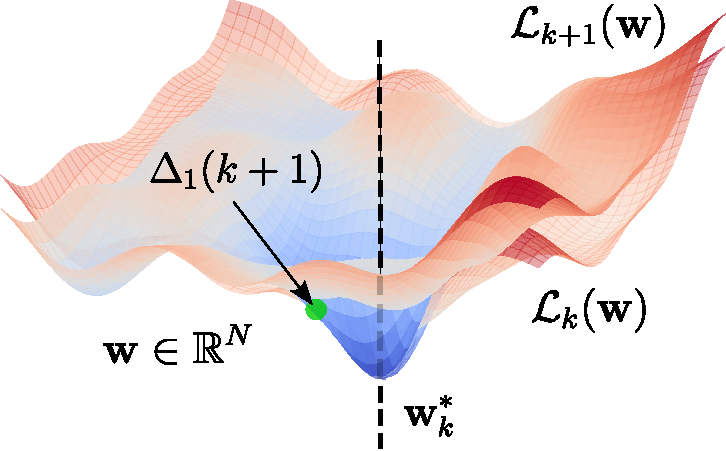
\includegraphics[width=\linewidth]{criterion_abs.pdf}\\[0.3em]
    \small (a) Absolute one-point criterion~$\Delta_1$
  \end{minipage}\hfill
  \begin{minipage}[t]{0.32\linewidth}
    \centering
    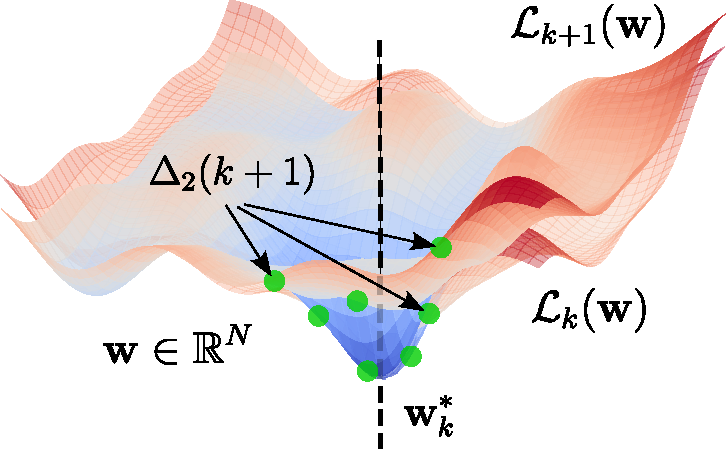
\includegraphics[width=\linewidth]{criterion_squared.pdf}\\[0.3em]
    \small (b) Full-space mean-squared criterion~$\Delta_2$
  \end{minipage}\hfill
  \begin{minipage}[t]{0.32\linewidth}
    \centering
    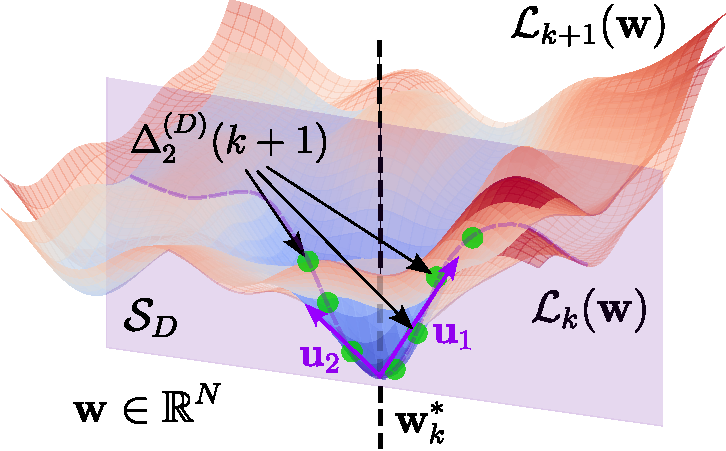
\includegraphics[width=\linewidth]{criterion_squared_subspace.pdf}\\[0.3em]
    \small (c) Subspace mean-squared criterion~$\Delta_2^{(D)}$
  \end{minipage}
  \caption{
  Schematic view of three observational designs for local landscape stabilization:
  (a) pointwise probing at a single location near $\mathbf w_k^*$;
  (b) isotropic mean-squared probing in the full parameter space;
  (c) mean-squared probing restricted to the principal curvature subspace.
  }
  \label{fig:criteria-overview}
\end{figure}

% \paragraph{Preview of the analysis.}
% The next section studies $\Delta_2^{(D)}$ under a local quadratic model of the increment field near $\mathbf w_k^*$.
% We show that the subspace criterion preserves the mean-squared $\mathcal O(k^{-2})$ decay of the full-space criterion and derive a low-dimensional representation of the increment in the principal curvature subspace.

\section{Theoretical analysis}
\label{sec:theory}

We analyze $\Delta_2^{(D)}$ through the local behavior of the increment field $\mathcal L_{k+1}(\mathbf w)-\mathcal L_k(\mathbf w)$ near $\mathbf w_k^*$.
Our goal is to derive a local quadratic representation of this field and to show that, under this model, the curvature-aware criterion preserves the same mean-squared $\mathcal O(k^{-2})$ decay as the full-space criterion.
Thus, the results below should be read as local guarantees for the subspace criterion rather than as global statements about the loss landscape.

\paragraph{Exact increment under one-sample growth.}
Adding one training example $(\mathbf x_{k+1}, \mathbf y_{k+1})$ to $\mathfrak D_k = \{(\mathbf x_i, \mathbf y_i)\}_{i=1}^k$ gives the exact identity
\begin{equation}
\label{eq:loss-increment-exact}
\mathcal L_{k+1}(\mathbf w)-\mathcal L_k(\mathbf w)
=
\frac{1}{k+1}\Bigl(\ell_{k+1}(\mathbf w)-\mathcal L_k(\mathbf w)\Bigr).
\end{equation}
Thus, local landscape stabilization can be studied through the decay of the deformation induced by one additional sample.

\paragraph{Local quadratic model.}
Fix $\mathbf w_0\in\mathbb R^N$ and assume that $\mathcal L_k$ and $\mathcal L_{k+1}$ are twice continuously differentiable in a neighborhood of $\mathbf w_0$.
Using second-order Taylor expansions at $\mathbf w_0$, we write
\begin{equation}
\label{eq:taylor-quadratic}
\mathcal L_m(\mathbf w)
\approx
\mathcal L_m(\mathbf w_0)
+
\mathbf g^{(m)}(\mathbf w_0)^\top(\mathbf w-\mathbf w_0)
+
\frac12(\mathbf w-\mathbf w_0)^\top \mathbf H^{(m)}(\mathbf w_0)(\mathbf w-\mathbf w_0),
\end{equation}
where
\[
\mathbf g^{(m)}(\mathbf w)=\nabla_{\mathbf w}\mathcal L_m(\mathbf w),
\qquad
\mathbf H^{(m)}(\mathbf w)=\nabla_{\mathbf w}^2\mathcal L_m(\mathbf w).
\]
Subtracting the quadratic expansions of $\mathcal L_{k+1}$ and $\mathcal L_k$ at the same reference point yields the local quadratic model of the increment field:
\begin{multline}
\label{eq:loss-diff-second}
\mathcal L_{k+1}(\mathbf w)-\mathcal L_k(\mathbf w)
\approx
\mathcal L_{k+1}(\mathbf w_0)-\mathcal L_k(\mathbf w_0)
\\
+
\Bigl(\mathbf g^{(k+1)}(\mathbf w_0)-\mathbf g^{(k)}(\mathbf w_0)\Bigr)^\top(\mathbf w-\mathbf w_0)
\\
+
\frac12(\mathbf w-\mathbf w_0)^\top
\Bigl(\mathbf H^{(k+1)}(\mathbf w_0)-\mathbf H^{(k)}(\mathbf w_0)\Bigr)
(\mathbf w-\mathbf w_0).
\end{multline}
All results below are derived for this local quadratic model rather than for the exact increment outside the approximation regime.

\paragraph{Centering at a minimizer of $\mathcal L_k$.}
Set $\mathbf w_0=\mathbf w_k^*$, where $\mathbf w_k^*$ is a local minimizer of $\mathcal L_k$.
Since $\mathbf g^{(k)}(\mathbf w_k^*)=\mathbf 0$, \eqref{eq:loss-diff-second} becomes
\begin{multline}
\label{eq:loss-diff-minimum}
\mathcal L_{k+1}(\mathbf w)-\mathcal L_k(\mathbf w)
\approx
\underbrace{\mathcal L_{k+1}(\mathbf w_k^*)-\mathcal L_k(\mathbf w_k^*)}_{\text{value gap}}
\\
+
\underbrace{\mathbf g^{(k+1)}(\mathbf w_k^*)^\top(\mathbf w-\mathbf w_k^*)}_{\text{gradient mismatch}}
+
\underbrace{\frac12(\mathbf w-\mathbf w_k^*)^\top
\Bigl(\mathbf H^{(k+1)}(\mathbf w_k^*)-\mathbf H^{(k)}(\mathbf w_k^*)\Bigr)
(\mathbf w-\mathbf w_k^*)}_{\text{curvature mismatch}}.
\end{multline}
This decomposition drives the subspace reduction and rate analysis below.

\paragraph{Subspace-supported observation of the increment.}
Under the local quadratic model \eqref{eq:loss-diff-minimum}, restricting probing to any $D$-dimensional subspace $\mathcal S(\mathbf V)=\operatorname{Im}(\mathbf V)$ ($\mathbf V\in\mathbb R^{N\times D}$ orthonormal) reduces the increment to a low-dimensional quadratic in the coordinate $\mathbf z$, where $\mathbf w=\mathbf w_k^*+\mathbf V\mathbf z$.
The resulting subspace criterion $\Delta_2^{(\mathbf V)}$ is therefore entirely determined by three compressed objects:
\[
a_k = \mathcal L_{k+1}(\mathbf w_k^*)-\mathcal L_k(\mathbf w_k^*),
\quad
\mathbf c_{k,\mathbf V} = \mathbf V^\top \mathbf g^{(k+1)}(\mathbf w_k^*),
\quad
\mathbf B_{k,\mathbf V} = \mathbf V^\top \mathbf A_k \mathbf V,
\]
where $\mathbf A_k=\mathbf H^{(k+1)}(\mathbf w_k^*)-\mathbf H^{(k)}(\mathbf w_k^*)$.
We specialize to the Hessian eigenspaces of $\mathbf H^{(k)}(\mathbf w_k^*)$ because they provide a spectral basis for the local quadratic geometry of $\mathcal L_k$ at $\mathbf w_k^*$, making the resulting criterion interpretable in terms of curvature modes.

\begin{lemma}[Reduction on the principal curvature subspace]
\label{lem:subspace-reduction}
Let $\mathbf U_D=[\mathbf u_1,\dots,\mathbf u_D]\in\mathbb R^{N\times D}$ contain the top-$D$ eigenvectors of $\mathbf H^{(k)}(\mathbf w_k^*)$, and set $\mathbf c_k=\mathbf U_D^\top\mathbf g^{(k+1)}(\mathbf w_k^*)$, $\mathbf B_k=\mathbf U_D^\top\mathbf A_k\mathbf U_D$.
Suppose $\operatorname{supp}(q)\subset (\mathbf w_k^*+\mathcal S_D)\cap \mathcal U_R(\mathbf w_k^*)$.
Under the parameterization $\mathbf w=\mathbf w_k^*+\mathbf U_D\mathbf z$, the distribution $q$ induces $\tilde q$ on $\mathbb R^D$, and
\begin{equation}
\label{eq:subspace-reduction-integral}
\Delta_2^{(D)}(k+1)
=
\int_{\mathbb R^D}
\left(
a_k + \mathbf c_k^\top \mathbf z + \frac12 \mathbf z^\top \mathbf B_k \mathbf z
\right)^2
\, \tilde q(\mathbf z) d\mathbf z.
\end{equation}
\end{lemma}

Here $\mathbf B_k$ is the compression of the Hessian difference $\mathbf A_k$ to the principal curvature subspace.
In general, $\mathbf B_k$ need not be diagonal, since the eigenvectors of $\mathbf H^{(k)}(\mathbf w_k^*)$ need not be eigenvectors of $\mathbf H^{(k+1)}(\mathbf w_k^*)$.

\paragraph{Rate bound for the principal-subspace criterion.}
Under the local quadratic model, the principal-subspace criterion preserves the same mean-squared $\mathcal O(k^{-2})$ decay as the full-space criterion, with the curvature-dependent term scaling through the subspace dimension $D$.

\begin{theorem}[Subspace mean-squared rate]
\label{thm:subspace-rate}
Suppose Lemma~\ref{lem:subspace-reduction} applies and that the per-example bounds
\[
\|\mathbf g_{k+1}(\mathbf w_k^*)\|_2 \le M_{\mathbf g},
\qquad
|\ell_i(\mathbf w_k^*)| \le M_\ell,
\qquad
\|\mathbf H_i(\mathbf w_k^*)\|_2 \le M_{\mathbf H}
\]
hold for $i=1,\dots,k+1$.
Let $\tilde q(\mathbf z)=\mathcal N(\mathbf 0,\sigma^2\mathbf I_D)$.
Then
\begin{equation}
\label{eq:subspace-rate-bound}
\Delta_2^{(D)}(k+1)
\le
\frac{
12M_\ell^2
+
3\sigma^2 M_{\mathbf g}^2
+
3\sigma^4(D^2+2D)M_{\mathbf H}^2
}{(k+1)^2}
=
\mathcal O(k^{-2}).
\end{equation}
\end{theorem}

Thus the rate matches the full-space mean-squared criterion, while the curvature-dependent term scales with $D$ rather than the ambient dimension $N$.

\paragraph{Spectral interpretation under stable principal directions.}
The rate bound above does not require any alignment between the eigenspaces of $\mathbf H^{(k)}(\mathbf w_k^*)$ and $\mathbf H^{(k+1)}(\mathbf w_k^*)$.
For interpretation, we now isolate the special case in which the leading directions remain stable.

\begin{assumption}[Stable principal directions (optional)]
\label{ass:stable-principal}
The eigenvectors $\mathbf u_1,\dots,\mathbf u_D$ associated with the $D$ largest eigenvalues of $\mathbf H^{(k)}(\mathbf w_k^*)$ are also eigenvectors of $\mathbf H^{(k+1)}(\mathbf w_k^*)$:
\[
\mathbf H^{(k+1)}(\mathbf w_k^*)\,\mathbf u_i
=
\lambda_i^{(k+1)}\mathbf u_i,
\qquad i=1,\dots,D.
\]
\end{assumption}

Under Assumption~\ref{ass:stable-principal},
\[
\mathbf B_k
=
\operatorname{diag}\bigl(
\lambda_1^{(k+1)}-\lambda_1^{(k)},
\dots,
\lambda_D^{(k+1)}-\lambda_D^{(k)}
\bigr).
\]

\begin{corollary}[Spectral closed form under vanishing linear and value terms]
\label{cor:spectral}
Suppose Assumption~\ref{ass:stable-principal} holds, $\tilde q(\mathbf z)=\mathcal N(\mathbf 0,\sigma^2\mathbf I_D)$, and $a_k=0$, $\mathbf c_k=\mathbf 0$.
Then
\begin{equation}
\label{eq:spectral-closed-form}
\Delta_2^{(D)}(k+1)
=
\frac{\sigma^4}{4}
\left(
2\sum_{i=1}^D (\lambda_i^{(k+1)}-\lambda_i^{(k)})^2
+
\left(
\sum_{i=1}^D (\lambda_i^{(k+1)}-\lambda_i^{(k)})
\right)^2
\right).
\end{equation}
\end{corollary}

This gives a direct spectral expression for the subspace criterion in the stable-eigenspace regime.

\paragraph{Why the top-curvature subspace?}
The next lemma provides a restricted extremality statement within the family of eigenspace-aligned subspaces.

\begin{lemma}[Extremality of the top-curvature subspace]
\label{lemma:extremal-topD}
Assume that $a_k=0$, $\mathbf c_k=\mathbf 0$.
Suppose that $\mathbf H^{(k)}(\mathbf w_k^*)$ and $\mathbf H^{(k+1)}(\mathbf w_k^*)$ are simultaneously diagonalizable with a common orthonormal eigenbasis $\{\mathbf u_i\}_{i=1}^N$, and let $\delta_i=\lambda_i^{(k+1)}-\lambda_i^{(k)}$, $i=1,\dots,N$. Assume further that $\delta_1 \ge \delta_2 \ge \cdots \ge \delta_N \ge 0$.
For any index set $I\subset\{1,\dots,N\}$ with $|I|=D$, let $\mathcal S_I=\operatorname{span}\{\mathbf u_i:\ i\in I\}$,
and define the corresponding quadratic subspace criterion by restricting \eqref{eq:delta2-subspace-method} to $\mathbf w_k^*+\mathcal S_I$ under the local quadratic model, with Gaussian coordinates $\mathbf z\sim\mathcal N(\mathbf 0,\sigma^2\mathbf I_D)$.
Then
\begin{equation}
\label{eq:extremal-criterion}
\Delta_{2,I}^{\mathrm{quad}}(k+1)
=
\frac{\sigma^4}{4}
\left(
2\sum_{i\in I}\delta_i^2
+
\left(\sum_{i\in I}\delta_i\right)^2
\right),
\end{equation}
and the maximum over all index sets $I$ with $|I|=D$ is attained at $I^*=\{1,\dots,D\}$.
Equivalently, the top-$D$ eigenspace of $\mathbf H^{(k)}(\mathbf w_k^*)$ maximizes the pure quadratic stabilization signal within the eigenspace-aligned family.
\end{lemma}

Lemma~\ref{lemma:extremal-topD} is restricted to the pure quadratic regime and to eigenspace-aligned subspaces.
It does not address linear or value terms, eigenspace drift, or arbitrary $D$-dimensional subspaces.
Its role is to provide an interpretable justification of the top-$D$ choice within this aligned family.

\section{Algorithmic estimation at scale}
\label{sec:algo}

The subspace criterion $\Delta_2^{(D)}$ gives rise to two distinct estimation targets.
One may estimate the \emph{true} criterion itself, defined through the original loss increment restricted to the principal curvature subspace, or its \emph{quadratic surrogate}, obtained by replacing the true increment with
\[
a_k + \mathbf c_k^\top \mathbf z + \frac12 \mathbf z^\top \mathbf B_k \mathbf z.
\]
All subspace-based estimators considered below share the same two-stage structure:
first, construct the principal curvature subspace at $\mathbf w_k^*$; second, estimate either the true criterion or its quadratic surrogate within that subspace.

\paragraph{Cost notation.}
Let $C_{\mathrm{fwd}}(m)$ denote the cost of one forward evaluation of $\mathcal L_m(\mathbf w)$, $C_{\mathrm{bwd}}(m)$ the cost of one backward pass, and $C_{\mathrm{HVP}}(m)$ the cost of one Hessian--vector product with $\mathbf H^{(m)}(\mathbf w)$.
We write $S$ for the number of Monte Carlo samples, $D$ for the subspace dimension, and $T_{\mathrm{eig}}$ for the number of eigensolver iterations.

\paragraph{Stage I: principal curvature subspace.}
For each $k$, we construct the principal curvature subspace at $\mathbf w_k^*$ by computing the top-$D$ eigenvectors of $\mathbf H^{(k)}(\mathbf w_k^*)$ using HVP-based iterative eigensolvers such as Lanczos or LOBPCG~\citep{pearlmutter1994fast}.
If each iteration requires $\mathcal O(D)$ HVPs, the total cost is
\[
\mathcal O\!\bigl(T_{\mathrm{eig}}\,D\,C_{\mathrm{HVP}}(k)\bigr).
\]
This is a one-time setup cost per value of $k$ shared by all subspace-based estimators.

\paragraph{Direct estimation of the true subspace criterion.}
Sampling
\[
\mathbf z_s \sim \mathcal N(\mathbf 0,\sigma^2\mathbf I_D),
\qquad
\mathbf w_s=\mathbf w_k^*+\mathbf U_D\mathbf z_s,
\qquad
s=1,\dots,S,
\]
gives the Monte Carlo estimator
\begin{equation}
\label{eq:direct-subspace-mc}
\widehat{\Delta}_{2,\mathrm{dir}}^{(D)}(k+1)
=
\frac{1}{S}\sum_{s=1}^S
\Bigl(
\mathcal L_{k+1}(\mathbf w_s)-\mathcal L_k(\mathbf w_s)
\Bigr)^2.
\end{equation}
This estimator targets the true criterion $\Delta_2^{(D)}$ and does not rely on the quadratic approximation.
Its total cost is
\[
\mathcal O\!\left(
S\bigl(
ND + C_{\mathrm{fwd}}(k)+C_{\mathrm{fwd}}(k+1)
\bigr)
\right),
\]
typically dominated by the two forward evaluations per sample.

\paragraph{Quadratic surrogate estimators.}
Under the local quadratic model from Section~\ref{sec:theory}, the increment in the principal curvature subspace is approximated by
\[
a_k + \mathbf c_k^\top \mathbf z + \frac12 \mathbf z^\top \mathbf B_k \mathbf z,
\]
where
\[
a_k = \mathcal L_{k+1}(\mathbf w_k^*)-\mathcal L_k(\mathbf w_k^*),\qquad
\mathbf c_k = \mathbf U_D^\top \mathbf g^{(k+1)}(\mathbf w_k^*),
\]
and
\[
\mathbf B_k
=
\mathbf U_D^\top
\bigl(
\mathbf H^{(k+1)}(\mathbf w_k^*)-\mathbf H^{(k)}(\mathbf w_k^*)
\bigr)
\mathbf U_D.
\]
Thus the surrogate is fully determined by the compressed coefficients $(a_k,\mathbf c_k,\mathbf B_k)$.
Their one-time assembly cost is
\begin{equation}
\label{eq:proxy-setup-cost}
\mathcal O\!\left(
C_{\mathrm{fwd}}(k)+C_{\mathrm{fwd}}(k+1)
+
C_{\mathrm{bwd}}(k+1)
+
D(C_{\mathrm{HVP}}(k)+C_{\mathrm{HVP}}(k+1))
+
ND^2
\right).
\end{equation}

\paragraph{Quadratic Monte Carlo.}
Replacing the true increment in \eqref{eq:direct-subspace-mc} by its quadratic surrogate gives
\begin{equation}
\label{eq:quad-subspace-mc}
\widehat{\Delta}_{2,\mathrm{quadMC}}^{(D)}(k+1)
=
\frac{1}{S}\sum_{s=1}^S
\left(
a_k + \mathbf c_k^\top \mathbf z_s + \frac12 \mathbf z_s^\top \mathbf B_k \mathbf z_s
\right)^2,
\qquad
\mathbf z_s \sim \mathcal N(\mathbf 0,\sigma^2\mathbf I_D).
\end{equation}
After the setup cost \eqref{eq:proxy-setup-cost}, this estimator costs
\[
\mathcal O(SD^2).
\]

\paragraph{Gaussian-moment estimator.}
Because the quadratic surrogate is a polynomial in $\mathbf z$ and the probing law is Gaussian, its expectation can be evaluated in closed form:
\begin{equation}
\label{eq:quad-closed-form}
\widehat{\Delta}_{2,\mathrm{GM}}^{(D)}(k+1)
=
\mathbb E_{\mathbf z\sim\mathcal N(\mathbf 0, \sigma^2 \mathbf I_D)}
\left[
\left(
a_k + \mathbf c_k^\top \mathbf z + \frac12 \mathbf z^\top \mathbf B_k \mathbf z
\right)^2
\right].
\end{equation}
Using the Gaussian moment identities from the proof of Theorem~\ref{thm:subspace-rate} yields
\begin{equation}
\label{eq:quad-closed-form-expanded}
\widehat{\Delta}_{2,\mathrm{GM}}^{(D)}(k+1)
=
a_k^2
+
a_k \sigma^2 \operatorname{Tr}(\mathbf B_k)
+
\sigma^2 \|\mathbf c_k\|_2^2
+
\frac{\sigma^4}{4}
\left(
2\operatorname{Tr}(\mathbf B_k^2)
+
\operatorname{Tr}(\mathbf B_k)^2
\right).
\end{equation}
After setup, evaluating this estimator costs
\[
\mathcal O(D^2).
\]

\paragraph{Full-space baseline.}
For comparison, the full-space mean-squared criterion $\Delta_2$ can be estimated by
\begin{equation}
\label{eq:fullspace-mc}
\widehat{\Delta}_{2,\mathrm{full}}(k+1)
=
\frac{1}{S}\sum_{s=1}^S
\Bigl(
\mathcal L_{k+1}(\mathbf w_k^*+\boldsymbol{\xi}_s)
-
\mathcal L_k(\mathbf w_k^*+\boldsymbol{\xi}_s)
\Bigr)^2,
\qquad
\boldsymbol{\xi}_s \sim \mathcal N(\mathbf 0,\sigma^2\mathbf I_N).
\end{equation}
Its cost is
\[
\mathcal O\!\Bigl(
S\bigl(
N + C_{\mathrm{fwd}}(k)+C_{\mathrm{fwd}}(k+1)
\bigr)
\Bigr),
\]
again typically dominated by the two forward evaluations per sample.

\paragraph{Summary of trade-offs.}
Table~\ref{tab:estimator-summary} summarizes the estimators considered in this section.
Direct subspace Monte Carlo estimates the true criterion and is therefore the most faithful estimator of $\Delta_2^{(D)}$.
Quadratic Monte Carlo and the Gaussian-moment estimator are cheaper after setup, but they target only the quadratic surrogate rather than the original criterion.
Their comparison in Section~\ref{sec:experiments} therefore tests not only computational trade-offs, but also the fidelity of the local quadratic model itself.

\begin{table}[t]
\caption{Summary of estimators for local landscape stabilization criteria}
\label{tab:estimator-summary}
\begin{center}
\small
\begin{tabular}{p{3.0cm} p{2.5cm} p{2.0cm} p{3.0cm}}
\toprule
\multicolumn{1}{c}{\bf Estimator} &
\multicolumn{1}{c}{\bf Target quantity} &
\multicolumn{1}{c}{\bf Additional quantities} &
\multicolumn{1}{c}{\bf Cost after subspace construction}
\\
\midrule
Full-space Monte Carlo baseline
&
true $\Delta_2$
&
none
&
$\mathcal O\!\left(S\bigl(N + C_{\mathrm{fwd}}(k)+C_{\mathrm{fwd}}(k+1)\bigr)\right)$
\\[0.5em]

Direct subspace Monte Carlo
&
true $\Delta_2^{(D)}$
&
$\mathbf U_D$
&
$\mathcal O\!\left(S\bigl(ND + C_{\mathrm{fwd}}(k)+C_{\mathrm{fwd}}(k+1)\bigr)\right)$
\\[0.5em]

Quadratic Monte Carlo
&
quadratic surrogate of $\Delta_2^{(D)}$
&
$a_k,\mathbf c_k,\mathbf B_k$
&
setup cost $+\ \mathcal O(SD^2)$
\\[0.5em]

Gaussian-moment estimator
&
quadratic surrogate of $\Delta_2^{(D)}$
&
$a_k,\mathbf c_k,\mathbf B_k$
&
setup cost $+\ \mathcal O(D^2)$
\\
\bottomrule
\end{tabular}
\end{center}
\end{table}

\section{Experiments}\label{sec:experiments}

\paragraph{Setup.}
All experiments use the nanochat depth-6 model (tag~\texttt{d6}) evaluated at training step~3500.
The nanochat architecture is a decoder-only transformer with rotary position embeddings, grouped-query attention, $\mathrm{ReLU}^2$ activations, and RMSNorm without learnable parameters.
Hessian--vector products are computed in float32 precision using the SDPA math kernel to ensure numerical stability of second-order computations.
Unless stated otherwise, we use $k=8$ sequences to define $\mathcal{L}_k$ and $\mathcal{L}_{k+1}$, and construct the top-$D$ Hessian subspace via deflated power iteration at $\mathbf{w}_k^*$.

\paragraph{Quadratic proxy validity.}
Before using any proxy-based estimator, we identify the perturbation scales $\sigma$ at which the local quadratic model \eqref{eq:taylor-quadratic} is reliable.
For a fixed checkpoint $\mathbf{w}_k^*$, we draw isotropic Gaussian perturbations $\boldsymbol{\delta}\sim\mathcal{N}(\mathbf{0},\sigma^2\mathbf{I}_N)$ and compare the true increment $\mathcal{L}_k(\mathbf{w}_k^*+\boldsymbol{\delta})-\mathcal{L}_k(\mathbf{w}_k^*)$ to its second-order Taylor approximation $\mathbf{g}^{(k)\top}\boldsymbol{\delta}+\frac{1}{2}\boldsymbol{\delta}^\top\mathbf{H}^{(k)}\boldsymbol{\delta}$.
The mean relative error, averaged over multiple random seeds, is plotted in Fig.~\ref{fig:exp-1} over $\sigma\in[10^{-7},10^{-1}]$.
The approximation error is never exactly zero due to higher-order contributions, but is reliably small for $\sigma\lesssim10^{-3}$.
All proxy-based estimators are therefore restricted to this regime in subsequent experiments.

\begin{figure}[t]
    \centering
    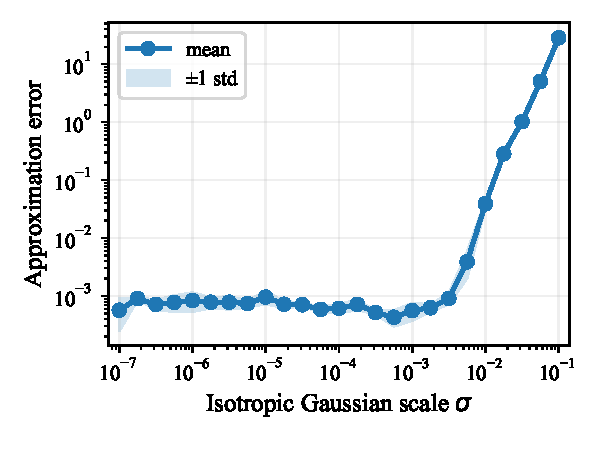
\includegraphics[width=0.7\linewidth]{quadratic_sigma_loggrid_1e7_1e1_plot_abs.pdf}
    \caption{Relative error of the quadratic Taylor approximation vs.\ perturbation scale $\sigma$ (mean and standard deviation across seeds, nanochat \texttt{d6} model, step~3500). The quadratic model is reliable for $\sigma\lesssim10^{-3}$; this regime defines the valid operating range for proxy-based estimators.}
    \label{fig:exp-1}
\end{figure}

\paragraph{Estimator comparison.}
Table~\ref{tab:exp-2} reports wall-clock times (seconds; mean $\pm$ sample std over five seeds) for the three estimators of Section~\ref{sec:algo} on the nanochat \texttt{d6} model, decomposed into three pipeline stages.
Stage~I constructs the principal curvature subspace by computing the top-$D$ eigenvectors of $\mathbf{H}^{(k)}(\mathbf{w}_k^*)$ via HVP-based power iteration; this stage is shared by all three estimators and dominates the total wall time.
Stage~II assembles the compressed proxy coefficients $(a_k, \mathbf{c}_k, \mathbf{B}_k)$ via one backward pass and $2D$ Hessian--vector products; it is required only by the two proxy estimators (marked \textemdash{} for Direct~MC).
Stage~III is the criterion evaluation: MC sampling for Direct~MC and Quadratic~MC, or the $\mathcal{O}(D^2)$ closed-form Gaussian-moment identity.

After the shared Stage~I, the Gaussian-moment (GM) estimator is approximately $18{,}000\times$ faster than Direct MC in Stage~III ($0.12\,\mathrm{ms}$ vs.\ $2.20\,\mathrm{s}$), making it the most efficient option once the subspace has been constructed.

\begin{table}[t]
\caption{Wall-clock times (seconds; mean $\pm$ sample std over five seeds) for three estimators of $\Delta_2^{(D)}$ on the nanochat \texttt{d6} model ($D=45$, step~3500). Stage~I: top-$D$ Hessian eigenvectors (shared). Stage~II: gradient and compressed Hessian assembly (proxy estimators only). Stage~III: criterion evaluation.}
\label{tab:exp-2}
\begin{center}
\small
\begin{tabular}{p{3.0cm} p{2.5cm} p{2.0cm} p{3.0cm}}
    \toprule
    \multicolumn{1}{c}{\bf Estimator} &
    \multicolumn{1}{c}{\bf Stage I (s)} &
    \multicolumn{1}{c}{\bf Stage II (s)} &
    \multicolumn{1}{c}{\bf Stage III (s)}
    \\
    \midrule
    Direct MC      & $17.53 \pm 0.53$ & \textemdash{} & $2.197 \pm 0.013$ \\
    Quadratic MC   & $17.53 \pm 0.53$ & $1.777 \pm 0.014$ & $(3.68 \pm 0.05)\times10^{-3}$ \\
    Gaussian moment & $17.53 \pm 0.53$ & $1.777 \pm 0.014$ & $(1.22 \pm 0.03)\times10^{-4}$ \\
    \bottomrule
\end{tabular}
\end{center}
\end{table}

Fig.~\ref{fig:exp-3} shows Direct~MC and Quadratic~MC estimates of $\widehat{\Delta}_2^{(D)}$ as functions of the Monte Carlo sample count~$S$, at fixed $D=10$ and $\sigma=10^{-3}$, with the GM closed form as a horizontal reference.
Both MC estimators converge to the GM value as $S$ increases, confirming that the GM estimator is the zero-variance limit of Quadratic~MC.

\begin{figure}[t]
    \centering
    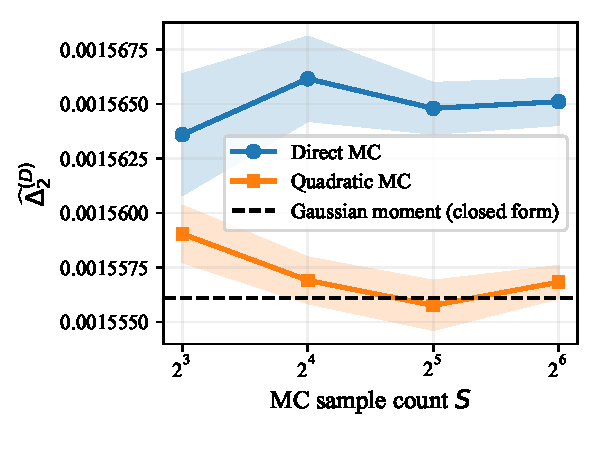
\includegraphics[width=0.7\linewidth]{delta2_robustness_d6_3500_D10sigma1e3_scurve.pdf}
    \caption{Convergence of Direct~MC (blue) and Quadratic~MC (orange) estimates of $\widehat{\Delta}_2^{(D)}$ to the Gaussian-moment closed form (dashed) as the sample count $S$ increases, at $D=10$, $\sigma=10^{-3}$ (nanochat \texttt{d6}, step~3500). Shaded bands show $\pm1$ standard error.}
    \label{fig:exp-3}
\end{figure}

Fig.~\ref{fig:exp-4} shows the relative error $|\widehat{\Delta}_{\mathrm{direct}}-\mathrm{GM}|/(|\widehat{\Delta}_{\mathrm{direct}}|+\varepsilon)$ as a heatmap over subspace dimension $D\in[1,100]$ and scale $\sigma\in[10^{-7},10^{-2}]$.
Within the valid proxy regime ($\sigma\lesssim10^{-3}$), the relative error is small across all tested subspace dimensions, confirming that the GM estimator serves as an accurate and computationally efficient surrogate for Direct~MC in practice.

\begin{figure}[t]
    \centering
    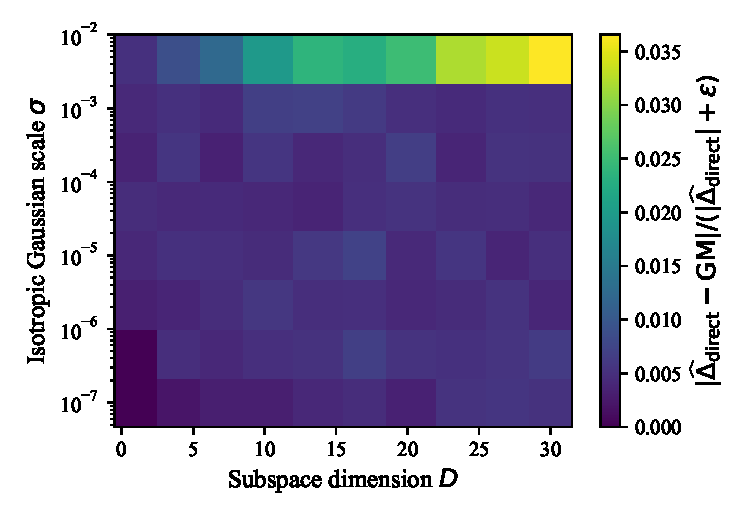
\includegraphics[width=0.7\linewidth]{delta2_robustness_d6_3500_D10sigma1e3_heatmap.pdf}
    \caption{Relative error $|\widehat{\Delta}_{\mathrm{direct}}-\mathrm{GM}|/(|\widehat{\Delta}_{\mathrm{direct}}|+\varepsilon)$ over subspace dimension $D\in[1,100]$ and perturbation scale $\sigma\in[10^{-7},10^{-2}]$ (nanochat \texttt{d6}, step~3500, $S=24$ MC samples per cell). Within the valid proxy regime ($\sigma\lesssim10^{-3}$), the relative error is small across all~$D$, showing that the GM estimator is robust to the choice of subspace dimension.}
    \label{fig:exp-4}
\end{figure}

\section{Discussion and limitations}
\label{sec:discussion}

The main contribution of this paper is not a new asymptotic law, but a unified framework for local stabilization criteria and a curvature-aware way of probing the increment field under sample growth.
The theory shows that the subspace criterion is compatible with the same mean-squared $\mathcal O(k^{-2})$ regime as the full-space criterion under a local quadratic model, but it does not imply universal optimality of the top-curvature subspace.

The main limitations are also clear.
First, the analysis is local: all guarantees are derived under a quadratic approximation near $\mathbf w_k^*$.
Second, although the top-curvature subspace is geometrically natural, the experiments show that at the tested perturbation scales different subspace families remain empirically similar because the scalar value-gap term dominates the criterion.
Third, the quadratic proxy estimators are accurate only in an extremely local regime, which makes direct subspace Monte Carlo the more reliable estimator in practice.

Our experiments also remain limited in scope: they establish the picture on a single nanochat decoder-only transformer rather than across architectures and domains.
More broadly, the paper suggests that stabilization criteria should be understood not only through what they aggregate, but also through how they probe local landscape change.
Natural next steps are to design criteria that suppress the scalar value-gap term, develop richer local surrogates beyond the quadratic approximation, and test the same framework in larger and more diverse models.

\section{Conclusion}
\label{sec:conclusion}

We introduced a unified framework for local loss-landscape stabilization under sample growth and studied a curvature-aware mean-squared criterion obtained by restricting probing to the top-$D$ eigenspace of the empirical Hessian near a trained solution.

Under a local quadratic model, we showed that this criterion preserves the same mean-squared $\mathcal O(k^{-2})$ decay as the full-space criterion, with curvature dependence scaling through the subspace dimension $D$.
We also derived a spectral special case and described scalable estimators for both the true criterion and its quadratic surrogate.

Empirically, on nanochat, the GM estimator faithfully tracks Direct~MC across all tested subspace dimensions $D\in[1,100]$ and perturbation scales in the valid quadratic regime.
At the same time, quadratic proxy estimators are reliable only in an extremely local regime ($\sigma\lesssim10^{-3}$), beyond which the GM estimator diverges from Direct~MC.

Taken together, these results position $\Delta_2^{(D)}$ as a well-defined curvature-aware observable of local landscape stabilization and clarify both its usefulness and its limits.


%%%%%%%%%%%%%%%%%%%%%%%%%%%%%%%%%%%%%%%%%%%%%%%%%%%%%%%%%%%%


\bibliographystyle{unsrtnat}
\bibliography{references}


%%%%%%%%%%%%%%%%%%%%%%%%%%%%%%%%%%%%%%%%%%%%%%%%%%%%%%%%%%%%

\appendix

\section{Proofs}
\label{app:proofs}

\allowdisplaybreaks

\subsection{Proof of Lemma~\ref{lem:subspace-reduction}}

Since the columns of $\mathbf U_D\in\mathbb R^{N\times D}$ are orthonormal, every point of $\mathbf w_k^*+\mathcal S_D$ has a unique representation $\mathbf w=\mathbf w_k^*+\mathbf U_D\mathbf z$, $\mathbf z\in\mathbb R^D$.
Substituting into the local quadratic model \eqref{eq:loss-diff-minimum} and using $\mathbf g^{(k)}(\mathbf w_k^*)=\mathbf 0$:
\begin{align*}
\mathcal L_{k+1}(\mathbf w)-\mathcal L_k(\mathbf w)
&=
a_k
+
\mathbf g^{(k+1)}(\mathbf w_k^*)^\top \mathbf U_D\mathbf z
+
\frac12(\mathbf U_D\mathbf z)^\top \mathbf A_k (\mathbf U_D\mathbf z)
=
a_k + \mathbf c_k^\top \mathbf z + \frac12 \mathbf z^\top \mathbf B_k \mathbf z.
\end{align*}
Under the parameterization $\mathbf w=\mathbf w_k^*+\mathbf U_D\mathbf z$, the density $q$ supported on $\mathbf w_k^*+\mathcal S_D$ induces a density $\tilde q$ on $\mathbb R^D$.
Integrating yields \eqref{eq:subspace-reduction-integral}.

\subsection{Proof of Theorem~\ref{thm:subspace-rate}}

By Lemma~\ref{lem:subspace-reduction},
\[
\Delta_2^{(D)}(k+1)
=
\mathbb E_{\tilde q(\mathbf z)}
\left[
\left(
a_k+\mathbf c_k^\top\mathbf z+\frac12\mathbf z^\top\mathbf B_k\mathbf z
\right)^2
\right],
\qquad
\mathbf z\sim \mathcal N(\mathbf 0,\sigma^2\mathbf I_D).
\]
For any $x,y,z\in\mathbb R$,
\[
(x+y+z)^2\le 3(x^2+y^2+z^2),
\]
hence
\begin{equation}
\label{eq:app-thm-step1-new}
\Delta_2^{(D)}(k+1)
\le
3a_k^2
+
3\,\mathbb E\bigl[(\mathbf c_k^\top\mathbf z)^2\bigr]
+
\frac34\,\mathbb E\bigl[(\mathbf z^\top\mathbf B_k\mathbf z)^2\bigr].
\end{equation}

\paragraph{Zero-order term.}
Using \eqref{eq:loss-increment-exact} at $\mathbf w_k^*$,
\[
a_k
=
\mathcal L_{k+1}(\mathbf w_k^*)-\mathcal L_k(\mathbf w_k^*)
=
\frac{1}{k+1}\Bigl(\ell_{k+1}(\mathbf w_k^*)-\mathcal L_k(\mathbf w_k^*)\Bigr).
\]
Therefore
\[
|a_k|
\le
\frac{1}{k+1}
\Bigl(
|\ell_{k+1}(\mathbf w_k^*)|
+
|\mathcal L_k(\mathbf w_k^*)|
\Bigr).
\]
Moreover,
\[
|\mathcal L_k(\mathbf w_k^*)|
=
\left|
\frac1k\sum_{i=1}^k \ell_i(\mathbf w_k^*)
\right|
\le
\frac1k\sum_{i=1}^k |\ell_i(\mathbf w_k^*)|
\le
M_\ell,
\]
and also $|\ell_{k+1}(\mathbf w_k^*)|\le M_\ell$.
Hence
\begin{equation}
\label{eq:app-ak-sq-new}
|a_k|\le \frac{2M_\ell}{k+1},
\qquad
a_k^2\le \frac{4M_\ell^2}{(k+1)^2}.
\end{equation}

\paragraph{Linear term.}
Since $\mathbf g^{(k)}(\mathbf w_k^*)=\mathbf 0$,
\[
\mathbf b_k
=
\mathbf g^{(k+1)}(\mathbf w_k^*)
=
\frac{1}{k+1}\mathbf g_{k+1}(\mathbf w_k^*),
\qquad
\mathbf c_k=\mathbf U_D^\top\mathbf b_k.
\]
Because $\mathbf U_D$ has orthonormal columns,
\[
\|\mathbf c_k\|_2
\le
\|\mathbf U_D^\top\|_2\,\|\mathbf b_k\|_2
\le
\frac{M_{\mathbf g}}{k+1}.
\]
For $\mathbf z\sim\mathcal N(\mathbf 0,\sigma^2\mathbf I_D)$,
\begin{equation}
\label{eq:app-linear-new}
\mathbb E\bigl[(\mathbf c_k^\top\mathbf z)^2\bigr]
=
\mathbf c_k^\top \mathbb E[\mathbf z\mathbf z^\top]\mathbf c_k
=
\sigma^2\|\mathbf c_k\|_2^2
\le
\frac{\sigma^2 M_{\mathbf g}^2}{(k+1)^2}.
\end{equation}

\paragraph{Quadratic term.}
The matrix $\mathbf B_k$ is symmetric.
For $\mathbf z\sim\mathcal N(\mathbf 0,\sigma^2\mathbf I_D)$,
\begin{equation}
\label{eq:app-quad-moment-new}
\mathbb E\bigl[(\mathbf z^\top\mathbf B_k\mathbf z)^2\bigr]
=
2\sigma^4 \operatorname{Tr}(\mathbf B_k^2)
+
\sigma^4 \operatorname{Tr}(\mathbf B_k)^2.
\end{equation}
For symmetric $\mathbf B_k$,
\[
\operatorname{Tr}(\mathbf B_k^2)\le D\|\mathbf B_k\|_2^2,
\qquad
|\operatorname{Tr}(\mathbf B_k)|\le D\|\mathbf B_k\|_2,
\]
so
\begin{equation}
\label{eq:app-quad-bound-new}
\mathbb E\bigl[(\mathbf z^\top\mathbf B_k\mathbf z)^2\bigr]
\le
\sigma^4(D^2+2D)\|\mathbf B_k\|_2^2.
\end{equation}

Next,
\[
\|\mathbf B_k\|_2
=
\|\mathbf U_D^\top \mathbf A_k \mathbf U_D\|_2
\le
\|\mathbf U_D^\top\|_2\,\|\mathbf A_k\|_2\,\|\mathbf U_D\|_2
\le
\|\mathbf A_k\|_2.
\]
Using
\[
\mathbf H^{(m)}(\mathbf w_k^*)
=
\frac1m\sum_{i=1}^m \mathbf H_i(\mathbf w_k^*),
\]
we obtain
\begin{align*}
\mathbf A_k
&=
\mathbf H^{(k+1)}(\mathbf w_k^*)-\mathbf H^{(k)}(\mathbf w_k^*)
\\
&=
\frac{1}{k+1}\sum_{i=1}^{k+1}\mathbf H_i(\mathbf w_k^*)
-
\frac{1}{k}\sum_{i=1}^{k}\mathbf H_i(\mathbf w_k^*)
\\
&=
\frac{1}{k+1}
\Bigl(
\mathbf H_{k+1}(\mathbf w_k^*)-\mathbf H^{(k)}(\mathbf w_k^*)
\Bigr).
\end{align*}
Hence
\[
\|\mathbf A_k\|_2
\le
\frac{1}{k+1}
\Bigl(
\|\mathbf H_{k+1}(\mathbf w_k^*)\|_2
+
\|\mathbf H^{(k)}(\mathbf w_k^*)\|_2
\Bigr)
\le
\frac{2M_{\mathbf H}}{k+1},
\]
and therefore
\begin{equation}
\label{eq:app-B-bound-new}
\|\mathbf B_k\|_2\le \frac{2M_{\mathbf H}}{k+1},
\qquad
\mathbb E\bigl[(\mathbf z^\top\mathbf B_k\mathbf z)^2\bigr]
\le
\frac{4\sigma^4(D^2+2D)M_{\mathbf H}^2}{(k+1)^2}.
\end{equation}

\paragraph{Conclusion.}
Substituting \eqref{eq:app-ak-sq-new}, \eqref{eq:app-linear-new}, and \eqref{eq:app-B-bound-new} into \eqref{eq:app-thm-step1-new}, we obtain
\[
\Delta_2^{(D)}(k+1)
\le
\frac{
12M_\ell^2
+
3\sigma^2M_{\mathbf g}^2
+
3\sigma^4(D^2+2D)M_{\mathbf H}^2
}{(k+1)^2},
\]
which is exactly \eqref{eq:subspace-rate-bound}.

\subsection{Proof of Corollary~\ref{cor:spectral}}

Under the assumptions $a_k=0$ and $\mathbf c_k=\mathbf 0$, Lemma~\ref{lem:subspace-reduction} gives
\[
\Delta_2^{(D)}(k+1)
=
\frac14\,
\mathbb E\bigl[(\mathbf z^\top\mathbf B_k\mathbf z)^2\bigr],
\qquad
\mathbf z\sim\mathcal N(\mathbf 0,\sigma^2\mathbf I_D).
\]
Using \eqref{eq:app-quad-moment-new},
\[
\mathbb E\bigl[(\mathbf z^\top\mathbf B_k\mathbf z)^2\bigr]
=
2\sigma^4\operatorname{Tr}(\mathbf B_k^2)
+
\sigma^4\operatorname{Tr}(\mathbf B_k)^2.
\]
Under Assumption~\ref{ass:stable-principal},
\[
\mathbf B_k
=
\operatorname{diag}\bigl(
\lambda_1^{(k+1)}-\lambda_1^{(k)},
\dots,
\lambda_D^{(k+1)}-\lambda_D^{(k)}
\bigr).
\]
Therefore,
\[
\operatorname{Tr}(\mathbf B_k)
=
\sum_{i=1}^D \bigl(\lambda_i^{(k+1)}-\lambda_i^{(k)}\bigr),
\qquad
\operatorname{Tr}(\mathbf B_k^2)
=
\sum_{i=1}^D \bigl(\lambda_i^{(k+1)}-\lambda_i^{(k)}\bigr)^2.
\]
Substituting these identities into the previous display yields
\[
\Delta_2^{(D)}(k+1)
=
\frac{\sigma^4}{4}
\left(
2\sum_{i=1}^D (\lambda_i^{(k+1)}-\lambda_i^{(k)})^2
+
\left(
\sum_{i=1}^D (\lambda_i^{(k+1)}-\lambda_i^{(k)})
\right)^2
\right),
\]
which is exactly \eqref{eq:spectral-closed-form}.

\subsection{Proof of Lemma~\ref{lemma:extremal-topD}}

Fix an index set $I\subset\{1,\dots,N\}$ with $|I|=D$ and consider the eigenspace-aligned subspace
\[
\mathcal S_I=\operatorname{span}\{\mathbf u_i:\ i\in I\}.
\]
Under the assumptions of the lemma, the linear and value terms vanish, and the Hessian difference is diagonal in the common eigenbasis:
\[
\mathbf A_k
=
\mathbf H^{(k+1)}(\mathbf w_k^*)-\mathbf H^{(k)}(\mathbf w_k^*)
=
\sum_{i=1}^N \delta_i\, \mathbf u_i\mathbf u_i^\top,
\qquad
\delta_i=\lambda_i^{(k+1)}-\lambda_i^{(k)}.
\]
Let $\mathbf U_I$ denote the matrix whose columns are the vectors $\mathbf u_i$, $i\in I$.
Then the compressed Hessian difference on $\mathcal S_I$ is
\[
\mathbf B_{k,I}
=
\mathbf U_I^\top \mathbf A_k \mathbf U_I
=
\operatorname{diag}(\delta_i:\ i\in I).
\]
With Gaussian coordinates $\mathbf z\sim\mathcal N(\mathbf 0,\sigma^2\mathbf I_D)$, the local quadratic reduction (same argument as in Lemma~\ref{lem:subspace-reduction}, with $\mathbf U_D$ replaced by $\mathbf U_I$) and $a_k=0$, $\mathbf c_k=\mathbf 0$ give
\[
\Delta_{2,I}^{\mathrm{quad}}(k+1)
=
\frac14\,\mathbb E\bigl[(\mathbf z^\top \mathbf B_{k,I}\mathbf z)^2\bigr].
\]
Applying the Gaussian quadratic-form identity \eqref{eq:app-quad-moment-new},
\[
\mathbb E\bigl[(\mathbf z^\top \mathbf B_{k,I}\mathbf z)^2\bigr]
=
2\sigma^4 \operatorname{Tr}(\mathbf B_{k,I}^2)
+
\sigma^4 \operatorname{Tr}(\mathbf B_{k,I})^2.
\]
Since $\mathbf B_{k,I}$ is diagonal,
\[
\operatorname{Tr}(\mathbf B_{k,I}^2)=\sum_{i\in I}\delta_i^2,
\qquad
\operatorname{Tr}(\mathbf B_{k,I})=\sum_{i\in I}\delta_i.
\]
Therefore
\[
\Delta_{2,I}^{\mathrm{quad}}(k+1)
=
\frac{\sigma^4}{4}
\left(
2\sum_{i\in I}\delta_i^2
+
\left(\sum_{i\in I}\delta_i\right)^2
\right),
\]
which proves \eqref{eq:extremal-criterion}.

It remains to show that this quantity is maximized when $I=\{1,\dots,D\}$.
Define
\[
F(I)
=
2\sum_{i\in I}\delta_i^2
+
\left(\sum_{i\in I}\delta_i\right)^2.
\]
Since $\delta_1\ge\delta_2\ge\cdots\ge\delta_N\ge0$, both terms in $F(I)$ are monotone with respect to replacing a smaller selected $\delta_j$ by a larger unselected $\delta_i$.
More explicitly, suppose $i\notin I$, $j\in I$, and $\delta_i\ge \delta_j$, and define
\[
I'=(I\setminus\{j\})\cup\{i\}.
\]
Then
\[
\sum_{\ell\in I'}\delta_\ell
=
\sum_{\ell\in I}\delta_\ell - \delta_j + \delta_i
\ge
\sum_{\ell\in I}\delta_\ell,
\]
and similarly
\[
\sum_{\ell\in I'}\delta_\ell^2
=
\sum_{\ell\in I}\delta_\ell^2 - \delta_j^2 + \delta_i^2
\ge
\sum_{\ell\in I}\delta_\ell^2.
\]
Hence
\[
F(I')\ge F(I).
\]
By repeatedly exchanging smaller selected indices for larger unselected ones, one reaches the set $I^*=\{1,\dots,D\}$ without decreasing $F$.
Therefore $F(I)$, and hence $\Delta_{2,I}^{\mathrm{quad}}(k+1)$, is maximized at $I^*=\{1,\dots,D\}$.
This proves the lemma.

\section{Additional experimental details}
\label{app:exp}

\paragraph{Experimental settings.}
Our experiments use a run matrix rather than a single configuration.
The reference setting is a nanoGPT-style decoder-only transformer with $4$ layers, $4$ attention heads, embedding width $128$, and block length $64$, trained on Tiny Shakespeare with AdamW ($\beta_1=0.9$, $\beta_2=0.95$, weight decay $0.1$), learning rate $3\times 10^{-4}$, batch size $32$, and a fixed number of $20$ training epochs for each value of $k$.
The stronger setting follows the same overall protocol but uses a wider model, a longer context length, and the WikiText-2 training split as the text corpus.

\paragraph{Nested subsets and losses.}
For each sample size $k$, we fix a random ordering of the training pool and use the first $k$ examples, yielding nested subsets across $k$.
The empirical risk $\mathcal L_k$ is the mean next-token cross-entropy over all tokens in the corresponding subset.
All evaluations of $\mathcal L_k$ and $\mathcal L_{k+1}$ use the exact nested subsets associated with the given value of $k$.

\paragraph{Criteria and perturbation settings.}
For $\Delta_1$, we use $50$ random directions with perturbation scale $\varepsilon=0.02$.
For $\Delta_2$ and $\Delta_2^{(D)}$, the default setting uses $\sigma=0.02$ and $100$ Monte Carlo samples, together with the additional $\sigma$-sweeps reported in Section~\ref{sec:experiments}.
The subspace dimension is varied across the values reported in the main text.

\paragraph{Hessian-based quantities.}
Top-$D$ Hessian eigendirections are computed using Hessian--vector products and iterative eigensolvers, as described in Section~\ref{sec:algo}.
Unless stated otherwise, the principal curvature subspace is recomputed separately for each $k$.
When Hessian-based quantities are estimated on trimmed subsets for efficiency, this affects only the Hessian-based computations and is kept separate from the direct evaluation of the landscape criteria.

\paragraph{Seeds and sample-size grids.}
The reference Tiny Shakespeare experiments use three random seeds and the sample-size grid
\[
k \in \{100,150,200,300,400,500,700,1000,1500,2000,3000,4000,5000\}.
\]
The stronger WikiText-2 setting uses the grid reported in Section~\ref{sec:experiments}.

\paragraph{Recorded outputs.}
For each run, we record the main stabilization curves, $\sigma$-sweeps, comparisons across subspace families, eigenspace-overlap statistics, and estimator-comparison diagnostics.
All plots and summary statistics in the main text are generated from these recorded outputs.

\begin{table}[t]
  \centering
  \small
  \begin{tabular}{ll}
    \hline
    Setting & Values (reference range) \\
    \hline
    Architecture & nanoGPT-style decoder-only transformer \\
    Layers / heads / width & $4$ / $4$ / $128$ \\
    Block length & $64$ \\
    Optimizer & AdamW, $\beta_1=0.9$, $\beta_2=0.95$ \\
    Learning rate & $3\times 10^{-4}$ \\
    Weight decay & $0.1$ \\
    Batch size & $32$ \\
    Training budget & fixed $20$ epochs per $k$ \\
    MC samples $S$ & $100$ for $\Delta_2$ and $\Delta_2^{(D)}$ \\
    Default perturbation scale & $\sigma=0.02$ \\
    Hessian eigensolver budget & $30$ power iterations \\
    Random seeds & $3$ \\
    \hline
  \end{tabular}
  \caption{Reference experimental defaults for the Tiny Shakespeare setting.}
  \label{tab:exp-hparams}
\end{table}

%%%%%%%%%%%%%%%%%%%%%%%%%%%%%%%%%%%%%%%%%%%%%%%%%%%%%%%%%%%%

% \newpage
% \input{checklist.tex}


\end{document}